\subsection{Fases de una simulación}\label{header-n3}

Todos los problemas de CFD presentan la siguiente estructura: un módulo
de preproceso, otro de procesado y uno final de postproceso. Cada uno de
ellos responde a las siguientes funciones:

\subsubsection{Preprocesado}

\begin{itemize}
\item
  Definición de la geometría a modelizar (el dominio compuacional).
\item
  Generación de la malla o división del dominio en un número
  suficiente de celdas o elementos que no se superpongan y que cubran
  toda la geometría.
\item
  Identificación de los fenómenos físicos y químicos que pretenden
  modelarse.
\item
  Definición de las propiedades del fluido (o fluidos).
\item
  Especificación de las condiciones iniciales y de contorno del
  problema.
\end{itemize}

La generación de la malla es muy importante, porque condicionará
definitivamente la calidad de los resultados. En principio, cuanto más
fina sea la malla, más próxima a la solución real será la simulación.
Sin embargo, mallas extraordinariamente finas aumentan considerablemente
el tiempo de cálculo, por lo que siempre es necesario llegar a una
elección de compromiso. Además, un mallado eficiente siempre ha de ser
más fino en aquellas zonas donde se prevé un mayor gradiente en las
variables del flujo.

\subsubsection{Procesado}

Constituye la parte central del programa de resolución y es el
encargado de resolver de forma iterativa las ecuaciones que se han
activado previamente en el preproceso (los modelos). Aun siendo la
parte más importante, definido el código que se va a emplear y
configuradas las funciones adicionales para obtener los parametros
deseados durante la simulación (Ej. fuerza de arrastre, capa límite,
caudal de salida...), el usuario sólo tendrá que lanzar la ejecución y
esperar que los recursos computacionales de los que dispone resuelvan
el caso. Las ejecuciones, en función de los modelos y del tamaño de la
malla, pueden durar desde minutos hasta semanas o meses de cálculos en
tiempo real.

\subsubsection{Postprocesado}

Es una parte fundamental por cuanto permiten gestionar la ingente
cantidad de información que el código es capaz de generar. No sólo se
trata de disponer una interfaz gráfica, sino de una herramienta que
permita proporcionar variables integradas y promedidas para ofrecer
resultados globales. Esta fase Incluye una serie de herramientas
gráficas que permiten analizar los resultados:

\begin{itemize}
\item
  Representación gráfica del dominio y la malla (Salome, ParaView).
\item
  Mapas de contornos de las variables, planos de corte, trazas
  vectoriales, líneas de corriente, entre otras opciones de vista
  (ParaView).
\item
  Gráficas y distribuciones de las mediciones de las variables
  (Paraview con Python y Octave).
\item
  Renderizados de los resultados, animaciones con aparencia más
  realista (Blender).
\end{itemize}

\subsection{Herramientas para cada fase}\label{header-n52}

Las referencias para la elección de las herramientas más convenientes
para usuarios de OpenFOAM, depende de muchos factores, entre ellos el
critério personal y si el uso para el que están diseñadas es el más
acorde a lo que se requiere. A continuación, se presenta una breve guía
sobre las herramientas más comunes \footnote{\href{https://github.com/NanoSim/CoursesAndTrainingPortfolio/blob/master/3_EulerianModels/meshingTools.md}{Meshing
  Toools that Interface with OpenFOAM}}\footnote{\href{https://www.cfd-online.com/Wiki/Codes}{Codes}}\footnote{\href{https://www.cfd-online.com/Links/soft.html}{Links - Software}}\footnote{\href{https://www.reddit.com/r/CFD/comments/18ydig/best_opensource_mesh_program_for_use_with_openfoam/}{Best
  open-source mesh program for use with openFOAM}}.

\subsubsection{Preprocesado}\label{header-n68}

\paragraph{Generación del modelo}\label{header-n69}

\subparagraph{blockMesh\cite{OpenFOAM}}\label{header-n71}

Utilidad provista con OpenFOAM, apropiado para geometrías sencillas. El
usuario tendrá que definir los vértices, bloques y contornos del modelo;
así como, el número de celdas y la relación de grosores que tendrán.
Esto se define en un fichero con el nombre de \textbf{blockMeshDict},
ubicado en la carpeta \textless{}./system\textgreater{} del caso. Se
complica cuando se quieren superficies curvas
\footnote{\href{https://cfd.direct/openfoam/user-guide/plateHole/#x6-400002.2.1}{OpenFOAM
User Guide: 2.2 Stress analysis of plate with hole}}.

Adicionalmente, es posible automatizar la generación del fichero y
también se pueden utilizar otras herramientas que dispongan de interfaz
gráfica para visualizar y editar el contenido
\footnote{
\href{https://openfoamwiki.net/index.php/BlockMesh}{OpenFOAM
Wiki/BlockMesh}}.

\subparagraph{dynamicMeshDict\cite{Nozaki}}\label{header-n76}

En OpenFOAM, se pueden implementar movimientos en la malla y cambios en
la topología, con la funcionalidad \emph{Dynamic Mesh}, localizado en
\textless{}./constant\textgreater{}. En este diccionario, se define una
velocidad constante sobre el contorno que se quiere desplazar; y
habiendo definido los demás parámetros de entrada para el control del
movimiento de la malla, el movimiento se generará de manera automatizada
a lo largo del tiempo.

\subparagraph{snappyHexMes\cite{snappyHexMesh}}\label{header-n79}

Herramienta incluida en OpenFOAM, diseñada para generar mallas
hexaédricas sobre geometrías más complejas en fotmato STL. El proceso de
esta utilidad implica: crear una malla de base con blockMesh (tamaño de
celdas de nivel 0); sobre este dominio se incrusta la geometría del caso
(en STL); se lleva a cabo un refinado local de la malla base, en la
región comprendida por el modelo; después, se mueven los vertices de las
celdas, cercanas a los contornos de superficie; por último, eliminar las
celdas redundantes (el usuario deberá especificar un punto dentro del
modelo si es el flujo por el interior lo que se quiere estudiar, o fuera
si se quiere analizar el comportamiento del flujo entorno al modelo) y
descomponer en más capas (\emph{layers}) los contornos determinados.

Se dispone de una amplia documendación por la comunidad de usuarios
\footnote{\href{https://sites.google.com/site/snappywiki/snappyhexmesh/snappyhexmeshdict\#TOC-geometry}{snappyWiki}}
, detallando las instrucciones contenidas en el diccionario y los
parámetros a establecer, este fichero definirá el proceso al ejecutar la
utilidad \texttt{snappyHexMesh}
 \footnote{\href{https://www.youtube.com/watch?v=ObsFQUiVi1U}{OpenFOAM
  SnappyHexMesh Tutorial}}
\footnote{\href{https://openfoamwiki.net/images/f/f0/Final-AndrewJacksonSlidesOFW7.pdf}{A
  Comprehensive Tour of snappyHexMesh}}
\footnote{\href{http://hmf.enseeiht.fr/travaux/projnum/book/export/html/1467}{Mesh
  generation}}.

\paragraph{Geometría}\label{header-n94} \\

Para generar el arcivo \textbf{STL} se disponen varias alternativas:

\subparagraph{OpenSCAD\cite{OpenSCAD}}\label{header-n97}

Se trata de un lenguaje declarativo, multiplataforma, ofrece una
interfaz mínima y sencilla donde introducir un conjunto limitado de
funciones primitivas para generar sólidos en 3D de forma paramétrica.
Programa basado en la construcción de sólidos (\emph{Constructive Solid
Geometry}, CSG), lo cual evita errores de superficies mal conectadas.

Su estructura puede simplificarse en 3 categorías: formas (cubos,
cilindros, esferas); transformaciones (trasladas, girar, escalar,
simetría); y operaciones CSG (unión, diferencia, intersección)
\cite{iamwil}\cite{CheatSheet}\cite{howtoOpenSCAD} .

\subparagraph{FreeCAD\cite{FreeCAD}}\label{header-n109}

Programa para el modelado en 3D, paramétrico, dividido en áreas de
trabajo, permitiendo trabajar con las utilidades necesarias para el
desarrollo del modelo (partes sólidas, diseño de partes, bocetos).

Multiplataforma (Windows, Mac and Linux), capaz de leer y escribir
cantidad de formatos como STEP, IGES, STL, SVG, DXF, OBJ, IFC, DAE y
otros muchos.

\begin{itemize}
\item
  La elaboración del dibujo se puede definir en consola a partir de la
  definición de los puntos, ejemplo:

  \begin{itemize}
  \item
    \texttt{30,20}: coordenadas absolutas;
    \item
      \texttt{@0,-40}: coordenadas relativas;
    \item
      \texttt{50\textless{}30}: coordenadas polares;
    \item
      \texttt{@80\textless{}30}: coordenadas polares relativas.
   \end{itemize}

 \item
  Los parámetros de acotación de pueden editar desde
  \texttt{Current\ Drawing\ Preferences}, o desde el panel de la
  derecha, donde se definen la lista de capas, editando por capa las
  características de grosor de los trazos.
 \end{itemize}

\subparagraph{Blender\cite{Blender}}\label{header-n137}

Herramienta de código abierto usada para crear modelos y animaciones en
3D, bajo licencia GNU GPL. Se necesita tiempo de entrenamiento para
entender cómo manejarlo, así como, para hallar las opciones y atajos de
teclado más útiles para realizar el diseño.

Está desarrollada para artistas, por ello la mayoría de tutoriales se
centran en el renderizado. No obstante, siempre será necesario partir
por un modelo, luego resulta una herramienta útil para ambos fines.

Guía detallada sobre la herramienta: Blender 3D en la Educación\cite{Blender3DEd}.

Para crear imágenes o animaciones renderizadas, que se aproximen a la
visualización real del agua, a partir de los datos obtenidos de los casos:

\begin{itemize}
\item
  Blender Dynamic Paint: Make Real Time water\cite{youtubeBlenderWater}
\item
  Blender Tutorial - Everything You NEED to Know About Fluid Simulation!\cite{youtubeBlenderTutorial}
\item
  Advanced Post-Processing Introduction :: Blender\cite{youtubeBlenderTraining}
\item
  Blender Coupling Scripts\cite{BlenderCouplingScripts}
\end{itemize}


Complementos para Blender (escritos en lenguaje Python) que permiten
generar automáticamente el modelo (geometría y mallado) compatible para
OpenFOAM v2.6x\footnote{\href{https://openfoamwiki.net/index.php/Blender}{Blender with OpenFOAM}}:

\begin{itemize}
\item
  {[}Contrib/SwiftBlock{]} Complemento añadido en Blender para crear el
  diccionario \texttt{blockMeshDict}, permite al usuario crear la
  estructura de bloques hexaédrica como un objeto dentro de la interfaz
  ofrecida en Blender.
\item
  {[}Contrib/SwiftSnap{]} Otro complemento para Blender que actúa como
  guía para crear el diccionario snappyHexMesh, permitiendo al usuario
  total control sobre como y qué líneas proporcionar en los contornos,
  así como especificar el nombre de cada área, la configuración de
  resolución y las capas de malla.
\item
  SwiftSnap\cite{cfd-online} y
  swiftSnap\cite{swiftSnap} estas dos referencias aportan más información del
  uso de los complementos y detalles sobre la compatibilidad de la
  versión de OpenFOAM.
\end{itemize}

\paragraph{Generación del mallado}\label{header-n181}

OpenFOAM acepta la generacion de la malla mediante una gran variedad de
aplicaciones (mesh generators and CAD systems), con una orden directa
ejecutada desde la terminal. La tabla de software para los que se
dispone la conversion de la malla están enunciados en el siguiente
enlace \href{http://www.openfoam.org/features/mesh-conversion.php}{Mesh converters}.



Entre ellos, los más destacables son:

\subparagraph{Netgen\cite{Netgen}}\label{header-n190}

Software de código abierto para la generación de mallas teraédricas. No
está dirigido directamente para el CFD.

\begin{itemize}
\item
  NetGen User Manual\cite{netgen_usermanual}
\item
  CME-Netgen\cite{Netgen}
\item
  Meshing with Netgen\cite{Meshing_with_Netgen}
\item
  NGSolve, librería de elementos finitos para crear diferentes
  geometrías y mallas que podrán visualizarse con Netgen\cite{NETGEN_NGSolve}
\end{itemize}

\subparagraph{enGrit\cite{enGrit}}\label{header-n206}

Software de código abierto para la generación de mallas para el CFD.
Este utiliza las librerías de Netgen para mallas tetraédricas; y un
método desarrollado internamente para celdas prismáticas en la capa
límite.


\subparagraph{Salome\cite{Salome}}\label{header-n209}


Licencia GNU LGPL. Software que proporciona una plataforma genérica para
el pre- y postprocesado de simulaciones numéricas. Se basa en una
arquitectura abierta y flexible hecha con componentes reutilizables.


\begin{itemize}
\item
  Salome to OpenFOAM mesh conversion tutorial\cite{Salome_to_OpenFOAM}
\item
  CFD Online: mesh conversion Salome to OpenFOAM\cite{cfd-online_2}
\item
  CFD Online: boundary conditions and mesh exporting\cite{cfd-online_3}
\item
  Video Tutorial: Meshing With Body Fitting\cite{youtub_Meshing_With_Body_Fitting}
\item
  Salome body fitting for OpenFOAM case\cite{cfd-online_4}
\item
  Exporting a salome mesh to OpenFOAM\cite{Salome_mesh_to_OpenFOAM}
  \item
    Python script that exports a mesh to OpenFOAM\cite{salomeToOpenFOAM}
  \item
    {Salome OpenFOAM Tutorial-CAD model to Solution Complete\cite{youtube_Salome_OpenFOAM_Tutorial}
  \item
    CFMesh:feature definition or extraction in the .stl file: Salome gets too
    much time for boolean operations on native .stl files\cite{cfd-online_5}
  \end{itemize}

\subparagraph{cfMesh\cite{cfMesh}}\label{header-n242}


Proyecto extendido desde la Universidad de Zagreb. El proceso para
generar la malla es automatizado, controlado por el diccionario
\texttt{meshDict}, similar a la utilidad \texttt{snappyHexMesh} pero
permite definir refinados en los contornos de forma más simple. Está
desarrollado bajo licencia GPL, y compatible con todas las versiones
recientes de OpenFOAM. Los formatos aceptados para la geometría de
entrada son: fms, ftr, and stl.

\begin{itemize}
\item
  cfMesh está diseñado como una librería de algoritmos que realizan las
  tareas de mallado\footnote{\href{http://cfmesh.com/support-faq/}{Frequently
  Asked Questions}}  y permiten la personalización e implementación de
  varias características de mallado:
  \begin{itemize}
  \item
    Capaz de generar varios tipos de malla: Cartesiana (hexaedros) en 3D
    y 2D, poliédrica y tetraédrica.
  \item
    Requiere mucho menos esfuerzo manual que snappyHexMesh, y es 4-5
    veces más rápido. Permite una cobertura del 100\% de la capa límite.
  \item
    También está capacitado para generar mallas con +20 capas, activando
    la optimización de capas.
  \end{itemize}

\end{itemize}

\subparagraph{Gmesh\cite{geuzaine2009gmsh}}\label{header-n262}

Generador de mallas tridimensionales de elementos finitos, integrando
utilidades para el preproceso y postproceso.


\subparagraph{meshLab\cite{MeshLab}}\label{header-n265}

Código abierto para procesar y editar mallas tridimensionales.
Proporciona un conjunto de herramientas para editar, limpiar, corregir,
inspeccionar, renderizar, texturizar y convertir mallas. Ofrece
características para procesar datos producidos por otras herramientas y
sirve para preparar modelos para impresiones en 3D. (2016 Released)

\subsubsection{Procesado}\label{header-n269}

\paragraph{OpenFOAM\cite{OpenFOAM}}\label{header-n271}

OpenFOAM es un código CFD, de fuentes abiertas, de uso general. Está
escrito en C++, orientado a objetos, que lo hace más fácil de extender.
El paquete incluye módulos para una amplia gama de aplicaciones. FOAM
fue escrito por Henry Weller y otros en el Imperial Collage. Durante
unos años FOAM fue un código comercializado por la compañía Nabla. No
obstante, en 2004 decidieron lanzar el código bajo licencia GPL con el
nuevo nombre de OpenFOAM. Este se distribuyó por OpenCFD durante varios
años, pero en 2011 SGI compró OpenCFD. Después, SGI vendió OpenCFD y la
marca OpenFOAM a ESI Group en 2012. Henry y su equipo de OpenCFD ahora
trabajan para ESI Group y el código de OpenFOAM se sigue distribuyendo
gratuitamente bajo licencia GPL.

\paragraph{IHFOAM\cite{IHFOAM}}\label{header-n274}

Es un resolvedor desarrollado por el Instituto de Hidráulica Ambiental
de la Universidad de Cantabria
\footnote{\href{http://www.ihcantabria.com/es/}{IHCantabria}}, para flujos
bifásicos en 3D. Especialmente diseñado para simular procesos de
ingeniería hidráulica, costeros y offshore.

El paquete de IHFOAM incluye:

\begin{itemize}
\item
  La librería \emph{libIHWaveGeneration.so}, que añade condiciones de
  contorno individuales, \emph{alpha.water} y \emph{U}, para la
  generación de las olas.
\item
  La librería \emph{libIHwaveAbsorption.so}, que introduce las
  condiciones de contorno para la absorción pura de las olas aplicable
  al campo de velocidades. Fundado en teorías 2D o 3D, aplicables a
  casos en 3D.
\end{itemize}

\paragraph{SU2\cite{cfd-online_6}}\label{header-n286}

Código abierto creado en la Universidad de Stanford, es una colección de
herramientas de software escritas en C++ para realizar análisis de
Ecuaciones Diferenciales Parciales (Partial Differencial Equation, PDE)
y resolver problemas de optimización del límite PDE. El conjunto de
herramientas está diseñado pensando en la dinámica de fluidos
comutacional y la optimización de formas aerodinámicas, pero es
extensible para tratar conjuntos arbitrarios de ecuaciones de gobierno
como para la electrodinámica, flujos de reacciones químicas y muchos
otros.

\paragraph{REEF3D: Open-Source Hydrodynamics\cite{REEF3D}}\label{header-n289}

Enfocado a la ingeniería hidráulica, costera, mar abierto y ingeniería
ambiental. El uso del método de ajuste de niveles le permite calcular la
superficie libre de flujos complejos. El modelo se implementa en C ++
altamente modular y el código fuente está disponible bajo la licencia
GPL. La biblioteca MPI se usa para la paralelización. El modelo se
encuentra actualmente en desarrollo y se agregan características
adicionales a un ritmo acelerado. El objetivo es hacer la transición
completa de una herramienta de investigación a un poderoso software de
ingeniería.

\subsubsection{Post-procesado}\label{header-n292}

\paragraph{ParaView\cite{ParaView}}\label{header-n294}

Un postprocesador de vanguardia diseñado para poder manejar conjuntos de
grandes cantidades de datos. Distribuido como software de código
abierto, es altamente recomendable\cite{kitware_blog}
\cite{kitware_blog_1} \cite{UsingParaView} \cite{cfd-online_7}
\cite{wangbo}.

\paragraph{\texorpdfstring{
\href{http://www.gnuplot.info/}{gnuplot}}{gnuplot}}\label{header-n313}

Este software es una utilidad para graficar a través de línea de
comandos, portable para Linux, OS/2, MS Windows, OSX, VMS entre muchas
otras plataformas. El código fuente está protegido por derechos de autor
pero distribuido libremente. Originalmente fue creado para permitir a
científicos y estudiantes visualizar funciones matemáticas y datos de
forma interactiva, pero ha crecido para soportar muchos usos no
interactivos como el scripting web. También se utiliza como motor de
trazado para aplicaciones de terceros como Octave. Gnuplot ha sido
apoyado y ha estado en desarrollo activo desde 1986.

\begin{itemize}
\item
  \href{http://gnuplot.sourceforge.net/demo/}{Demos for gnuplot}
\item
  \href{http://gnuplot.sourceforge.net/demo_4.2/}{Demo scripts for
  gnuplot}
\item
  \href{http://people.duke.edu/~hpgavin/gnuplot.html}{GNUPLOT 4.2 - A
  Brief Manual and Tutorial}
\end{itemize}

\paragraph{\texorpdfstring{
\href{https://openfoamwiki.net/index.php/Contrib/PyFoam}{python}}{python}}\label{header-n326}

Python es un lenguaje interpretado, que permite crear aplicaciones para
controlar o modificar procesos. Existen unas librerías desarrolladas
para el control de la ejecución \emph{OpenFOAM-runs} y manipulación de
datos \emph{OpenFOAM-data}, de entre las que destacan las siguientes
utilidades:

\begin{itemize}
\item
  analizar los archivos de registro producidos por los resolvedores de
  OpenFoam;
\item
  ejecutar el resolvedor y las utilidades, analizando, simultáneamente,
  las salidas;
\item
  manipular los parámetros y condiciones iniciales de los archivos de
  forma no destructiva;
\item
  graficar los residuos del resolvedor.
\end{itemize}

Estas librerías se reunen en el paquete de \emph{PyFoam}, desarrolladas
para controlar las simulaciones de OpenFoam con script decentes para
realizar variaciones de parámetros o analizar resultados.

Referencias de interés para conocer más sobre el lenguaje:

\begin{itemize}
\item
  \href{https://openfoamwiki.net/index.php/Contrib/PyFoam\#Utilities_for_Logfiles}{Utilities
  for logfiles}
\item
  \href{http://www.learnpython.org/es/}{Training}
\item
  \href{https://openfoamwiki.net/index.php/File:ElevationVsTime.tar.gz}{File:ElevationVsTime.tar.gz}
\item
  \href{https://openfoamwiki.net/images/d/de/HappyFoamingWithPyFoam.pdf}{"Happy
  Foaming with Python"}
\item
  \href{http://web.student.chalmers.se/groups/ofw5/Advanced_Training/pyFoamAdvanced.pdf}{"Automatization
  with pyFoam"}
\end{itemize}

\paragraph{\texorpdfstring{
\href{http://pgfplots.sourceforge.net/}{PGFPlots}}{PGFPlots}}\label{header-n362}

Se trata de un paquete de LaTeX para crear gráficos de alta calidad con
escala normal o logarítmica en dos y tres dimensiones. Mediante unas
instrucciones sencillas, se define un gráfico con los datos del caso
contenidos en un archivo con formato \emph{dat}. Soporta gráficos de
líneas, de barras, áreas, diagramas de dispersión, histogramas, ejes
polares, diagramas ternarios, entre otros.

\subsubsection{Herramientas para el trabajo}\label{header-n366}

\paragraph{\texorpdfstring{
\href{http://engys.com/es/services/training}{helyx-os}}{helyx-os}}\label{header-n368}

HELYX-OS es una interfaz gráfica de usuario de código abierto, diseñada
para trabajar de forma nativa con OpenFOAM v4.1 and OpenFOAM v1606+.

En Engys combinan sus conocimiento de códigos comerciales con la amplia
experiencia de trabajo con herramientas de Código Abierto, para ofrecer
un portafolio variado de servicios de software CAE para la industria.

\begin{itemize}
\item
  \href{http://engys.com/es/products/helyx-os}{Ppales ventajas de
  HELYX-OS}

  \begin{itemize}
  \item
    Soporte nativo para librerías de archivos OpenFOAM.
  \item
    Plataformas para Linux y Windows.
  \item
    Control de la utilidad de mallado snappyHexMesh, incluyendo
    visualización de la geometría y ejecución de la utilidad a través de
    la interfaz.
  \item
    Módulo específico para la definición de modelos, incluyendo
    controles para turbulencia, transferencia de calor, condiciones de
    contorno, inicialización del flujo, ejecución del solver a través de
    la interfaz gráfica, etc.
  \end{itemize}
\item
  \href{http://engys.github.io/HELYX-OS//installation/}{HELYX-OS
  installation}

  \begin{itemize}
  \item
    El código fuente, los archivos binarios para Linux y las
    instrucciones de instalación para HELYX-OS.
  \end{itemize}
\end{itemize}

\paragraph{\texorpdfstring{
\href{https://www.docker.com/}{docker}}{docker}}\label{header-n397}

Se trata de una herramienta desarrollada para crear aplicaciones en
contenedores que luego se borrarán del sistema, ofreciendo la
posibilidad de arrancar la imagen del programa requerido, en el sistema
operativo seleccionado:\\

\begin{itemize}
\item
  Imágenes creadas por la comunidad y por los propios desarrolladores de
  algunos programas, las cuales se pueden descargar desde
  \href{https://hub.docker.com}{Docker Hub}.
\item
  Artículo que describe la imagen de OpenFOAM, para poder ser ejecutada
  desde Docker:
  \href{https://www.cfdengine.com/blog/how-to-install-openfoam-anywhere-with-docker/}{How
  to install OpenFOAM anywhere with Docker}.
\item
  \href{https://hub.docker.com/r/quantumhpc/openfoam/~/dockerfile/}{Dockerfile}
  es donde se guardan las instrucciones de lo que contiene el contenedor
  para crear la imagen a ejecutar. Es un archivo equivalente a un
  \emph{script}.
\item
  \href{http://stackoverflow.com/questions/32001523/docker-cant-write-to-directory-mounted-using-v-unless-it-has-777-permissions}{Docker
  can write to directory mounted}: Para compartir una carpeta del
  anfitrión con el contenedor, se necesita arrancar la imagen con el
  argumento \texttt{:Z}, de forma que se puedan saltar los permisos de
  seguridad de linux.
\end{itemize}

\paragraph{Travis}\label{header-n414}

Travis CI es un servidor que se sincroniza con los proyectos subidos a
GitHub para realizar automáticamente las pruebas del código que se hayan
implementado y guardarlas de forma comprimida en el repositorio.

Comunmente se usa para comprobaciones de códigos o cambios concretos en
el mismo, así como para revisar la compatibilidad con diferentes
entornos. Es decir, para la integración continua de modificaciones que
requieran verificar la ausencia de errores (\emph{test early}).

\subsection{Fases del experimento}\label{header-n420}

En un comienzo, se analizan las opciones existentes para ensayar el caso
con las maquetas disponibles del laboratorio, realizando varias
hipótesis sobre la definición del caso:

\begin{figure}
\centering
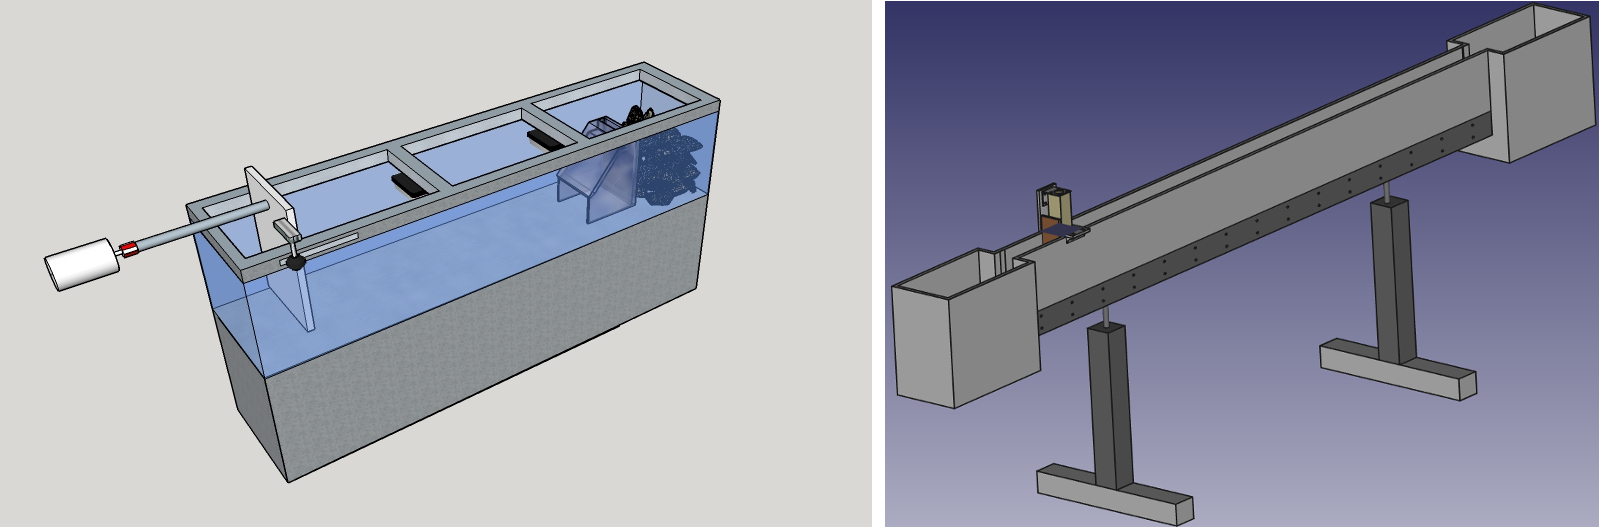
\includegraphics{11-tanqueCanal.jpg}
\caption{Tanque para la generación del oleaje y canal de corriente de agua}
\label{fig:tanqueCanal}
\end{figure}

Como el tanque no disponía, en su momento, del control del oleaje
debidamente caracterizado, y tampoco se conocían las posibilidades de
implementarlo en el modelo a analizar computacionalmente, se fue
desarrollando el caso de interés añadiendo modificaciones a los ejemplos
diseñados para resolverse desde OpenFOAM.

Asimismo, dada la complejidad que implica abordar cada fase de la
simulación, se descartó la posibilidad de incluir un oleaje continuo,
sustituyendose por una columna de agua retenida en el instante inicial
por una compuerta. Por ello, finalmente se optó por adaptar el canal a
una simulación del caso.

La representación del prototipo OWC, se lleva a cabo con la fabricación
de unas planchas de policarbonato, a medida del canal para crear la
cámara. Además, se coloca una tubería para que haga de chimenea, por
donde circulará el flujo de aire a compresión y succión, en función de
si el agua entra o sale de la cámara.

Por otro lado, se analizan las opciones de implementar una turbina del
tipo WELLS, comunmente utilizadas en estos casos para aprobechar el
flujo bidireccional. No obstante, como primer contacto con la ejecución
del CFD se consideró demasiado laborioso. Ya que computacionalmente
implicaría realizar un caso aparte, para venificar la aerodinámica de la
turbina, así como, caracterizar su funcionamiento para ciertas
condiciones de entrada. Del mismo modo, experimentalmente, también
resultaría una tarea complicada hallar la potencia real que se podría
obtener de ella. Por lo tanto, se sustituye por un diafragma del cual se
extraiga una potencia equivalente al punto de funcionamiento de una
turbina en concreto.

Con esta disposición, las mediciones que se realizan para hallar el
caudal del flujo de aire de salida y la potencia extraída, parten por
conocer el \emph{Coeficiente de caudal} en función de la relación de
áreas considerando el diámetro del diafragma entre el diámetro interior
del tubo (chimenea) y del número de Reynolds en el que se esté
trabajando. Debido a que el diámetro considerado para la chimenea es más
pequeño que lo que la norma establece para considerar un coeficiente ya
normalizado, se procede a caracterizar los diafragmas que se usarán en
el ensayo final.

Teniendo este valor, con conocer la presión estática aguas arriba del
diafragma, explicado con más detalle en el apartado /R/{[}4.Mediciones
experimentales{]}, será suficiente para hallar la potencia. Para medir
este valor en el ensayo final, se dispone de un \emph{Transductor de
presión} con un rango de mediciones de \(100Pa\) y \(\pm 25 Pa\), este
instrumento está conectado a un \emph{display} del cual no se conoce
cada cuánto realiza las lecturas. Sólo se sabe que estará condicionado
por l que el ojo humano es capaz de apreciar. Por ello, se realizará la
captura a través de una tarjeta de adquisición \emph{Labjack U3}, para
transferir estos valores a un ordenador. Las conexiones de la tarjeta de
adquisición se realizan con la ayuda de un profesor del laboratorio, así
como, la programación de estas lecturas a traves de \emph{LabVIEW}.

El desarrollo de las pruebas, implican establecer, primero, la condición
inicial del llenado de agua, midiendo con una regla la altura estimada.
Tras esto, se ejecuta el programa de \emph{LabVIEW} para accionar la
subida de la compuerta y capturar la presión estática máxima, lograda
cuando el agua entra en la cámara. Dadas, las fuertes reflexiones que se
experimentan y al no disponer de una generación continua de oleaje, la
energía de la primera ola originada, se reparte hasta estabilizarse. Es
por ello que sólo se analizará el primer ciclo de compresión del aire
dentro de la cámara y, no, el se succión.
